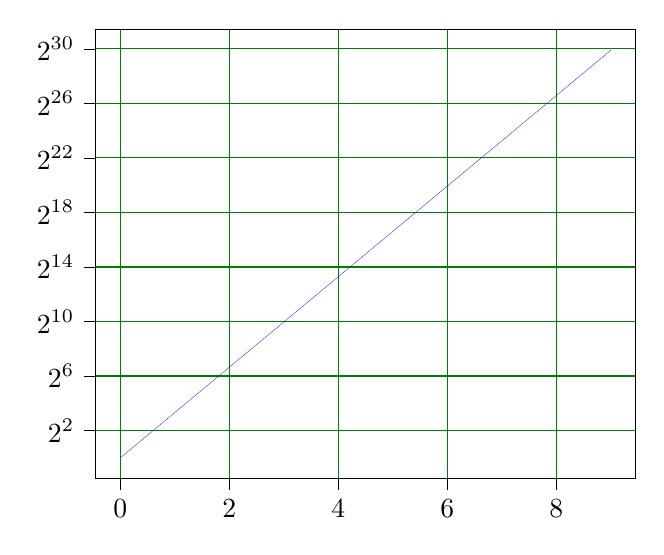
\begin{tikzpicture}

\definecolor{green01270}{RGB}{0,127,0}

\begin{axis}[
log basis y={2},
tick align=outside,
tick pos=left,
x grid style={green01270},
xmajorgrids,
xmin=-0.45, xmax=9.45,
xminorgrids,
xtick style={color=black},
y grid style={green01270},
ymajorgrids,
ymin=0.35481339, ymax=2.8183829e+09,
yminorgrids,
ymode=log,
ytick style={color=black},
ytick={0.015625,0.25,4,64,1024,16384,262144,4194304,67108864,1.0737418e+09,1.7179869e+10,2.7487791e+11},
yticklabels={
  \(\displaystyle {2^{-6}}\),
  \(\displaystyle {2^{-2}}\),
  \(\displaystyle {2^{2}}\),
  \(\displaystyle {2^{6}}\),
  \(\displaystyle {2^{10}}\),
  \(\displaystyle {2^{14}}\),
  \(\displaystyle {2^{18}}\),
  \(\displaystyle {2^{22}}\),
  \(\displaystyle {2^{26}}\),
  \(\displaystyle {2^{30}}\),
  \(\displaystyle {2^{34}}\),
  \(\displaystyle {2^{38}}\)
}
]
\addplot [ultra thin, blue]
table {%
0 1
1 10
2 100
3 1000
4 10000
5 100000
6 1000000
7 10000000
8 1e+08
9 1e+09
};
\end{axis}

\end{tikzpicture}
